\documentclass[12pt]{article}
\usepackage{natbib}
\usepackage{url}
\usepackage{stmaryrd}
\usepackage{mathrsfs}
\usepackage{amsmath}
\usepackage{graphicx}
\usepackage{parskip}
\usepackage{fancyhdr}
\usepackage{commath}%定义d
\usepackage[UTF8,scheme = plain]{ctex}
\usepackage{geometry}
\usepackage{bm}
\usepackage{siunitx}
\usepackage{float}
\usepackage{subfig}
\usepackage{titlesec}
\usepackage{caption}
\usepackage{paralist}
\usepackage{multirow}
\usepackage{booktabs} % To thicken table lines
\usepackage{diagbox}
\usepackage{authblk}
\usepackage{indentfirst}
\usepackage{amsthm}
\usepackage{fontspec}
\usepackage{color}
%\usepackage{txfonts} %设置字体为times new roman
\usepackage{lettrine}
\usepackage{nameref}
%\usepackage[nottoc]{tocbibind}
\usepackage{amssymb}%font
\usepackage{lipsum}%make test words
\usepackage{picinpar}%words around the picture
\usepackage[all]{xy}%draw arrow
\usepackage{asymptote}%draw picture
\usepackage[perpage]{footmisc}%脚注每页清零
\usepackage{esint}

\geometry{bottom=3cm,left=3cm,right=3cm,top=3cm}
% \footskip = 60pt

% \setmainfont{TimesNewRomanPSMT}
\setsansfont{Helvetica-Light}
\setCJKmainfont[ItalicFont=STKaitiSC-Regular,BoldFont=STSongti-SC-Black]{STSongti-SC-Regular}
\setCJKsansfont[BoldFont=STHeitiSC-Medium]{STHeitiSC-Light}


%\setmainfont{Times New Roman}

\ctexset{today=old}%日期类型设置

% ======================================
% = Color de la Universidad de Sevilla =
% ======================================
\usepackage{tikz}
\definecolor{PKUred}{cmyk}{0,1,1,0.45}

%超链接设置
\usepackage[breaklinks,colorlinks,linkcolor=PKUred,citecolor=PKUred,pagebackref,urlcolor=PKUred]{hyperref}
\usepackage{cleveref}
% \newcommand{\crefpairconjunction}{ 和 }


\newcommand{\hsp}{\hspace{20pt}}
\newcommand{\nhsp}{\hspace{-30pt}}
\titleformat{\section}{\Large\bfseries}{%\arabic{section}
\hspace{-22pt}\textcolor{PKUred}{\vrule width 2pt}\hsp}{0pt}{}


\titleformat{\subsection}
  {\normalfont\large\bfseries}{}{0em}{}

\renewcommand*\footnoterule{%
    \vspace*{-3pt}%
    {\color{PKUred}\hrule width 2in height 0.4pt}%
    \vspace*{2.6pt}%
}


%% Color the bullets of the itemize environment and make the symbol of the third
%% level a diamond instead of an asterisk.
%h\renewcommand*\textbullet{\dag}
\renewcommand*\labelitemi{\color{PKUred}\textbullet}
\renewcommand*\labelitemii{\color{PKUred}--}
\renewcommand*\labelitemiii{\color{PKUred}$\diamond$}
\renewcommand*\labelitemiv{\color{PKUred}\textperiodcentered}



%%% Equation and float numbering
\numberwithin{equation}{section}		% Equationnumbering: section.eq#
\numberwithin{figure}{section}			% Figurenumbering: section.fig#
\numberwithin{table}{section}				% Tablenumbering: section.tab#


%代码设置
\usepackage{listings}
\usepackage{fontspec} % 定制字体
\newfontfamily\menlo{SFMono-Regular}
\usepackage{xcolor} % 定制颜色
\definecolor{mygreen}{rgb}{0,0.6,0}
\definecolor{mygray}{rgb}{0.5,0.5,0.5}
\definecolor{mymauve}{rgb}{0.58,0,0.82}
\lstset{  
numbers=left,
numberstyle=\footnotesize\menlo,
basicstyle=\footnotesize\menlo,
backgroundcolor=\color{white},      % choose the background color
columns=fullflexible,
tabsize=4,
breaklines=true,               % automatic line breaking only at whitespace
captionpos=b,                  % sets the caption-position to bottom
commentstyle=\color{mygreen},  % comment style
escapeinside={\%*}{*)},        % if you want to add LaTeX within your code
keywordstyle=\color{blue},     % keyword style
stringstyle=\color{mymauve}\ttfamily,  % string literal style
frame=single,
rulesepcolor=\color{red!20!green!20!blue!20},
% identifierstyle=\color{red},
language=c++,
xleftmargin=4em,xrightmargin=2em, aboveskip=1em,
framexleftmargin=2em,
numbers=left
}

%脚注
\renewcommand\thefootnote{\fnsymbol{footnote}}

%定义常数i、e、积分符号d
\newcommand\mi{\mathrm{i}}
\newcommand\me{\mathrm{e}}

%%% Maketitle metadata
\newcommand{\horrule}[1]{\rule{\linewidth}{#1}} 	% Horizontal rule
\newcommand{\tabincell}[2]{\begin{tabular}{@{}#1@{}}#2\end{tabular}}


\setcounter{secnumdepth}{2}
\usepackage{bm}
\usepackage{autobreak}
\usepackage{amsmath}
\graphicspath{{../}}
\setlength{\parindent}{2em}
\newcommand{\bs}  [1]{\boldsymbol{#1}}

%pdf文件设置
\hypersetup{
	pdfauthor={袁磊祺},
	pdftitle={Advanced Fluid Mechanics Homework 4}
}

\title{
		\vspace{-1in} 	
		\usefont{OT1}{bch}{b}{n}
		\normalfont \normalsize \textsc{\LARGE Peking University}\\[1cm] % Name of your university/college \\ [25pt]
		\horrule{0.5pt} \\[0.5cm]
		\huge \bfseries{Advanced Fluid Mechanics Homework 4} \\
		\horrule{2pt} \\[0.5cm]
}
\author{
		\normalfont 								\normalsize
		College of Engineering \quad 2001111690  \quad 袁磊祺\\	\normalsize
        \today
}
\date{}

\begin{document}

%%%%%%%%%%%%%%%%%%%%%%%%%%%%%%%%%%%%%%%%%%%%%%
\captionsetup[figure]{name={图},labelsep=period}
\captionsetup[table]{name={表},labelsep=period}
\renewcommand\contentsname{目录}
\renewcommand\listfigurename{插图目录}
\renewcommand\listtablename{表格目录}
\renewcommand\refname{参考文献}
\renewcommand\indexname{索引}
\renewcommand\figurename{图}
\renewcommand\tablename{表}
\renewcommand\abstractname{摘\quad 要}
\renewcommand\partname{部分}
\renewcommand\appendixname{附录}
\def\equationautorefname{式}%
\def\footnoteautorefname{脚注}%
\def\itemautorefname{项}%
\def\figureautorefname{图}%
\def\tableautorefname{表}%
\def\partautorefname{篇}%
\def\appendixautorefname{附录}%
\def\chapterautorefname{章}%
\def\sectionautorefname{节}%
\def\subsectionautorefname{小小节}%
\def\subsubsectionautorefname{subsubsection}%
\def\paragraphautorefname{段落}%
\def\subparagraphautorefname{子段落}%
\def\FancyVerbLineautorefname{行}%
\def\theoremautorefname{定理}%
\crefname{figure}{图}{图}
\crefname{equation}{式}{式}
\crefname{table}{表}{表}
%%%%%%%%%%%%%%%%%%%%%%%%%%%%%%%%%%%%%%%%%%%

\maketitle

\section{1}

假设板宽为$l$,在\cref{fig:11}中, 板和水的相互作用力垂直与板, 虚线下的水和虚线上的水的相互作用力为竖直方向. 如\cref{fig:12}, 单位时间内水的动量改变量为
\begin{equation}
	\Delta \bm{p} = l\rho U d \Delta t (\bm{v_2}-\bm{v_1}),
\end{equation}
其中$\bm{v_2},\bm{v_1}$的大小为$U$, 方向和$\bm{p_2},\bm{p_1}$相同. 
由\cref{fig:12},
\begin{equation}
	\Delta \bm{p} = \Delta \bm{F}  \Delta t,
\end{equation}
其中
\begin{equation}
	\Delta \bm{F} = \bm{F_2} - \bm{F_1}.
\end{equation}
由几何关系可算得
\begin{equation}
	F = l\rho U d \cot \frac{\alpha}{2},
\end{equation}
所以滑板受到的水的总的垂直向上的支持力
\begin{equation}
	N = F \cos \alpha = l\rho U d \cot \frac{\alpha}{2} \cos \alpha.
\end{equation}
单位宽度滑板受到的水的总的垂直向上的支持力
\begin{equation}
	N' = \rho U d \cot \frac{\alpha}{2} \cos \alpha.
\end{equation}

\begin{figure}[htp]
	\centering
	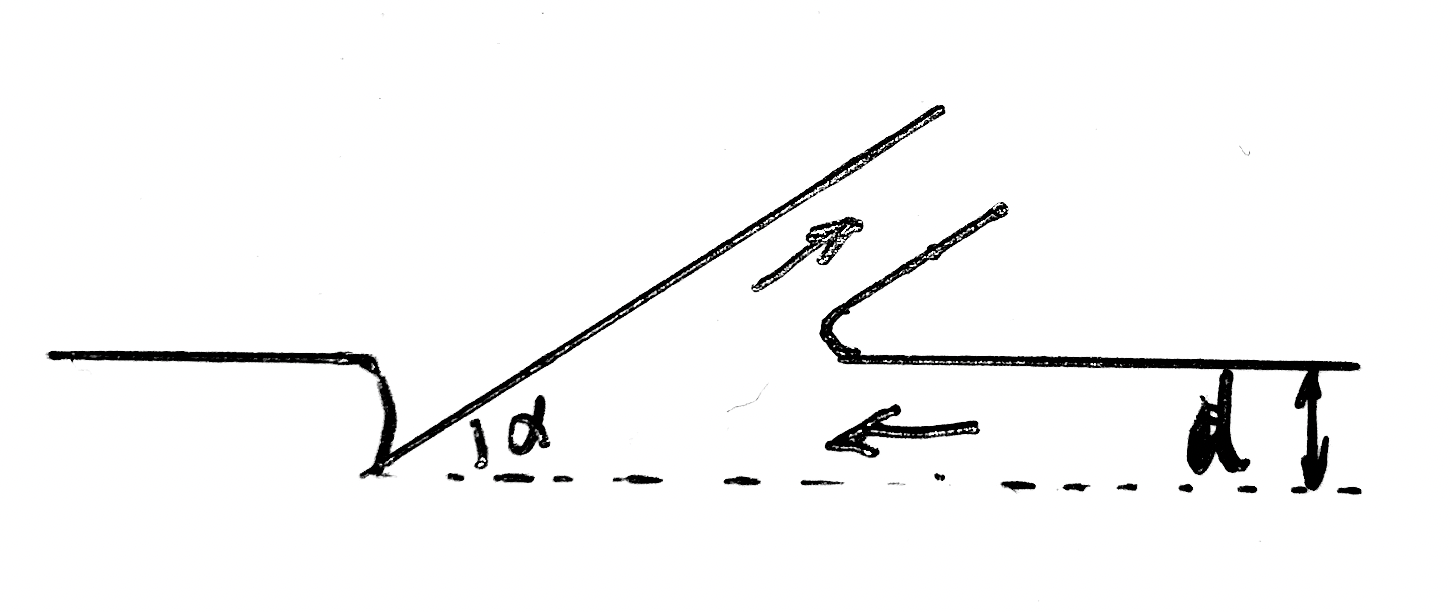
\includegraphics[width=12cm]{11.png}
	\caption{流动示意图}
	\label{fig:11}
\end{figure}

\begin{figure}[htp]
	\centering
	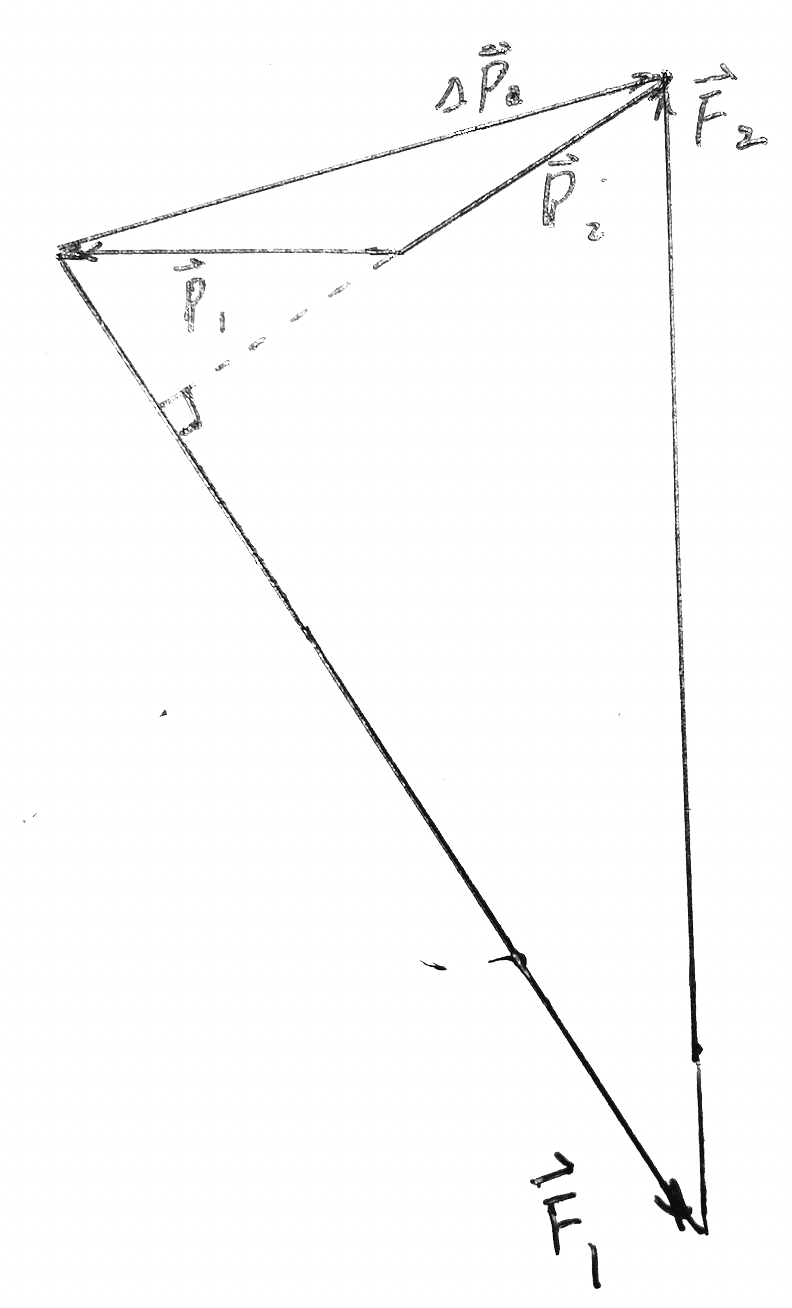
\includegraphics[width=5cm]{12.png}
	\caption{受力示意图}
	\label{fig:12}
\end{figure}

\section{2}

\subsection{(1)}

设液体密度为$\rho$,假设半径相同处的流体的流速基本相同. 取半径为$r$的控制体, 控制体内流体的总质量守恒,
\begin{equation}
	0 = \dif \ (\rho h \pi r^2) = r^2\dif h + 2hr\dif r,
\end{equation}
所以半径为$r$处流体的流速
\begin{equation}
	v(r) = \frac{\dif r}{\dif t} = - \frac{r}{2h} \frac{\dif h}{\dif t} = \frac{Ur}{2h}.
\end{equation}
半径从$r$到$r+\Delta r$处的流体受到上下板的阻力近似为
\begin{equation}
	\dif f(r) = \frac{v}{h} 2\pi r \dif r = \frac{\pi r^2U}{h^2}\dif r.
\end{equation}
不考虑流体的惯性力, $r$到$r+\Delta r$的压力差和阻力相等
\begin{equation}
	-2\pi rh\dif p(r) = \dif f(r) = \frac{\pi r^2U}{h^2}\dif r.
\end{equation}
\begin{equation}
	\dif p(r) = - \frac{rU}{2h^3}\dif r.
\end{equation}
假设流体外部压强为0, 则
\begin{equation}
	p(r) = \frac{U}{4h^3}\left(R^2-r^2\right).
\end{equation}
所以平板受到的阻力为
\begin{equation}
	F = \int_0^R 2\pi r p(r) \dif r = \int_0^R 2\pi r \frac{U}{4h^3}\left(R^2-r^2\right) \dif r = \frac{\pi U R^4}{8h^3}.
\end{equation}


\subsection{(2)}

考虑到液体表面张力的效应, 液体和空气的压强差
\begin{equation}
	\Delta p = \sigma \frac{1}{R},
\end{equation}
当$R$足够小时, $\Delta p$足够大, 液体可以支撑起平板. 


\section{3}

在考虑平板边界层时, 边界层是一个强剪切层, 当$\mathrm{Re}$趋于无穷时, 边界层就成为了面涡, 所以这里直接使用边界层厚度的结论
\begin{equation}
	\delta \approx \sqrt{\frac{\nu x}{U}} = \sqrt{\frac{x^2\rho}{\mathrm{Re}}},
\end{equation}
其中$x$是特征尺度, $U$是特征速度. 

\section{4}

引入这样一个环量函数, 假如我们考虑的点是面涡上的点A, 让环量函数穿过点A和面涡上的另一确定的点B, 其它路径任意, 则
\begin{equation}
	\oint_C \nabla \phi \cdot \dif \bm{x} = \llbracket \phi_A \rrbracket - \llbracket \phi_B \rrbracket \equiv \Gamma,
\end{equation}
所以
\begin{equation}
	\gamma = \bm{n} \times \nabla_\pi (\Gamma + \llbracket \phi_B \rrbracket) = \bm{n} \times \nabla_\pi \Gamma.
\end{equation}

\section{5}

根据Biot-Savart公式, 
\begin{equation}
	\boldsymbol{u}(\boldsymbol{x})=\frac{1}{2(n-1) \pi} \int_{S} \frac{\bm{\gamma}\left(\boldsymbol{x}^{\prime}\right) \times \boldsymbol{r}}{r^{n}} \dif S\left(\boldsymbol{x}^{\prime}\right).
\end{equation}
对于二维情况, 
\begin{equation}
	\boldsymbol{u}(\boldsymbol{x})=\frac{1}{2 \pi} \int_{S} \frac{\bm{\gamma}\left(\boldsymbol{x}^{\prime}\right) \times \boldsymbol{r}}{r^{2}} \dif l\left(\boldsymbol{x}^{\prime}\right).
\end{equation}
假设$\bm{\gamma}$的方向为垂直平面向上为$\bm{z}$, $\bm{\theta}$的方向为$\bm{z}\times \bm{r}$的方向. 由轴对称性, 速度只有$\bm{\theta}$方向的分量, 在环外
\begin{equation}
	u_\theta(r) 2 \pi r = \gamma 2 \pi a,
\end{equation}
\begin{equation}
	u_\theta(r) = \frac{\gamma a}{r}.
\end{equation}
其中$a$是面涡的半径, 在环内, $\bm{u}=0$.

对于面涡上的点, 
\begin{equation}
	u_\theta = \frac{\gamma a}{2r}.
\end{equation}
即圆形面涡绕圆心转圈, 所以该面涡的形状将不发生改变. \qed

\section{6}

$\bm{u}^+ = u^+_1 \bm{e}_1 + u^+_2 \bm{e}_2$ but $\bm{u}^− = u^−_1 \bm{e}_1$ for the velocities on the outer and inner sides of the sheet, respectively,
\begin{equation}
	\llbracket \boldsymbol{u} \rrbracket = \bm{u}^+ - \bm{u}^- = \left(u_{1}^{+}-u_{1}^{-}\right) \boldsymbol{e}_{1}+u_{2}^{+} \boldsymbol{e}_{2},
\end{equation}
\begin{equation}
	\overline{\boldsymbol{u}} = \frac{1}{2} \left(\bm{u}^+ + \bm{u}^-\right) = \frac{1}{2}\left[\left(u_{1}^{+}+u_{1}^{-}\right) \boldsymbol{e}_{1}+u_{2}^{+} \boldsymbol{e}_{2}\right],
\end{equation}
\begin{equation}
	\gamma = \bm{e}_3 \times \llbracket \boldsymbol{u} \rrbracket = u_{2}^{+} \boldsymbol{e}_{1}+\left(u_{1}^{-}-u_{1}^{+}\right) \boldsymbol{e}_{2},
\end{equation}
where
\begin{equation}
	\bm{e}_3 = \bm{e}_2 \times \bm{e}_1.
\end{equation}
\begin{equation}
	q^{+2} = 2 \overline{\boldsymbol{u}} \cdot \llbracket \boldsymbol{u} \rrbracket + u_{1}^{-2} = u_{1}^{+2}+u_{2}^{+2}=u_{1}^{-2}.
\end{equation}

\section{7}

\subsection{Birkhoff-Rott Equation}
Given vorticity, $\omega(\bs x)$, one can calculate the stream function, $\psi(\bs x)$ as follows:

\begin{equation}
\Delta \psi(\bs x) = \omega(\bs x)
\end{equation}
Now this can be solved to get
\begin{subequations}
\begin{align}
\psi(\bs x)&=\frac{1}{2\pi}\int\limits_D{\omega(\bs x)\ln|\bs x - \bs x'|}\\
\bs v(\bs x)&=\frac{1}{2\pi}\int\limits_D{\frac{\bs {\hat z}\times(\bs x - \bs x')}{|\bs x - \bs x'|^2}\omega(\bs x')d\bs x'}
\end{align}
Using $\omega(\bs x)d\bs x=d\Gamma(\bs x)$ and restricting the domain to be a curve $C$ we obtain   %=\Gamma'(\alpha)d\bs \alpha'$
\begin{align}
\frac{\partial x(\alpha,t)}{\partial t}& = \frac{-1}{2\pi} \int\limits_C{\frac{(y(\alpha,t)-y(\alpha',t))}{((x(t)-x(\alpha',t))^2 + (y(\alpha,t)-y(\alpha',t))^2 }}\Gamma'(\alpha')d\alpha'\\
\frac{\partial y(\alpha,t)}{\partial t} &= \frac{1}{2\pi}\int\limits_C{\frac{(x(t)-x(\alpha',t))}{((x(\alpha,t)-x(\alpha',t))^2 + (y(\alpha,t)-y(\alpha',t))^2 }}\Gamma'(\alpha')d\alpha'
\end{align}
\end{subequations}

\subsection{Desingularization of the Birkhoff-Rott equation}
Given $\delta>0$, called a smoothing parameter, we consider the equations:
\begin{subequations}
\label{mom}
\begin{align}
\frac{\partial x(\alpha,t)}{\partial t}& = \frac{-1}{2\pi} \int\limits_C{\frac{(y(\alpha,t)-y(\alpha',t))}{((x(t)-x(\alpha',t))^2 + (y(\alpha,t)-y(\alpha',t))^2 + \delta^2 }}\Gamma'(\alpha')d\alpha'\\
\frac{\partial y(\alpha,t)}{\partial t} &= \frac{1}{2\pi}\int\limits_C{\frac{(x(\alpha,t)-x(\alpha',t))}{((x(\alpha,t)-x(\alpha',t))^2 + (y(\alpha,t)-y(\alpha',t))^2 + \delta^2 }}\Gamma'(\alpha')d\alpha'\end{align}
\end{subequations}
These are called the $\delta$-equations, which is an approximation to the Birkhoff-Rott equation. Our goal here is to solve the $\delta$-equations numerically and observe its behaviour as $\delta$ approaches 0. 

\subsection{Discretization}

We apply standard discretization techniques to solve the $\delta$-equations.Let $z_j$(t)=$x_j$(t)+$iy_j$(t) be an approximation to the vortex sheet's position $z(\Gamma(\alpha_j),t)$ at equidistant parameter values $\alpha_j$=$\pi(j-1)/2N$ , $j=1,2.....2N+1$. The integral is evaluated by the trapezoidal rule, yielding a system of coupled ordinary differential equations for the blob's motions:

\begin{subequations}
\begin{align}
\frac{d x_j}{d t} = \sum_{k=1}^{2N+1}{\frac{-(y_j(t)-y_k(t))}{((x_j(t)-x_k(t))^2 + (y_j(t)-y_k(t))^2 + \delta^2)}}w_k\\
\frac{d y_j}{d t} = \sum_{k=1}^{2N+1}{\frac{(x_j(t)-x_k(t))}{((x_j(t)-x_k(t))^2 + (y_j(t)-y_k(t))^2 + \delta^2)}}w_k
\end{align}
\end{subequations}
where $w_k=\Gamma'(\alpha_k)\frac{1}{2\pi N},k=1,2.....2N+1$ refer to the quadrature weights. We use the fourth-order Runge Kutta scheme to integrate the above system of equations.
\subsection{Periodic Vortex Sheet}
The $\delta$-equations for a periodic vortex-sheet are given by:
\begin{subequations}
\begin{align}
\frac{d x_j}{d t}  =\frac{-1}{2N} \sum_{{\substack{k=1 \\ k\neq j}}}^{N}{\frac{\sinh2\pi(y_j(t)-y_k(t))}{(\cosh2\pi(x_j(t)-x_k(t)) - \cos2\pi(y_j(t)-y_k(t)) + \delta^2)}}w_k\\
\frac{d y_j}{d t}=\frac{1}{2N} \sum_{{\substack{k=1 \\ k\neq j}}}^{N}{\frac{\sin2\pi(x_j(t)-x_k(t))}{(\cosh2\pi(x_j(t)-x_k(t)) - \cos2\pi(y_j(t)-y_k(t)) + \delta^2)}}w_k
\end{align}
\end{subequations}
The initial conditions are given by
$x_j(0)=\Gamma_j+0.01\sin2\pi\Gamma_j$and $y_j(0)=-0.01\sin2\pi\Gamma_j$ . 

The figures below show a trignometric interpolating polynomial, in the variable $\Gamma$. It interpolates the perturbation quantities $p_j(t)=x_j(t)-\Gamma_j + iy_j(t)$, the coefficients of the polynomial are the fourier coefficients of $p_j$ and are calculated using the Fast Fourier Transform. The plotted image is $\Gamma + P(\Gamma,t)$, where P is the polynomial described above.








\begin{figure}[htp]
	\centering
	\subfloat{
	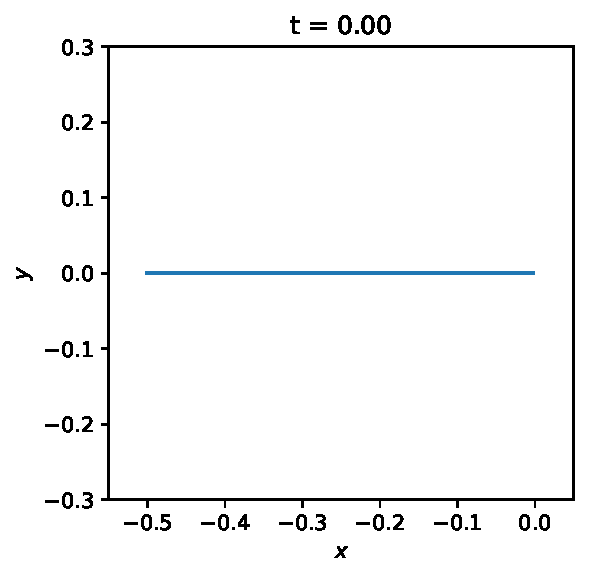
\includegraphics[width=7cm]{0.00.pdf}
	}\,
	\subfloat{
	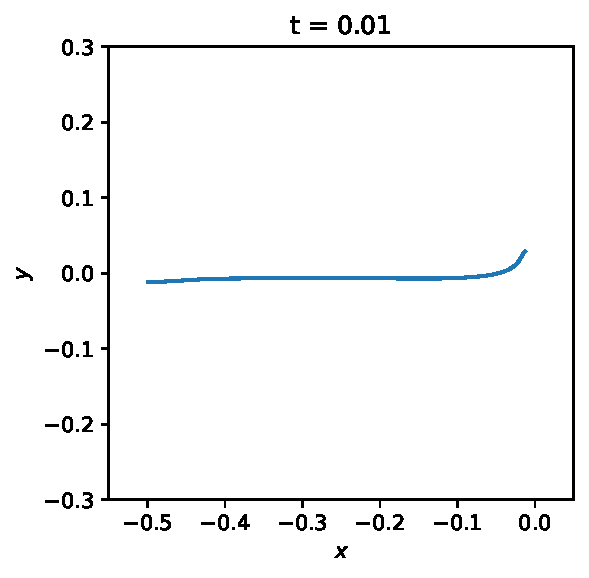
\includegraphics[width=7cm]{0.01.pdf}
	}\,
\end{figure}

\begin{figure}[htp]
	\centering
	\subfloat{
	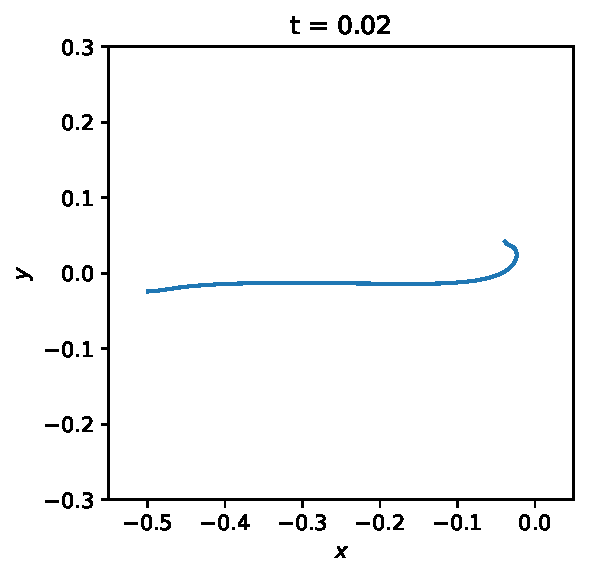
\includegraphics[width=7cm]{0.02.pdf}
	}\,
	\subfloat{
	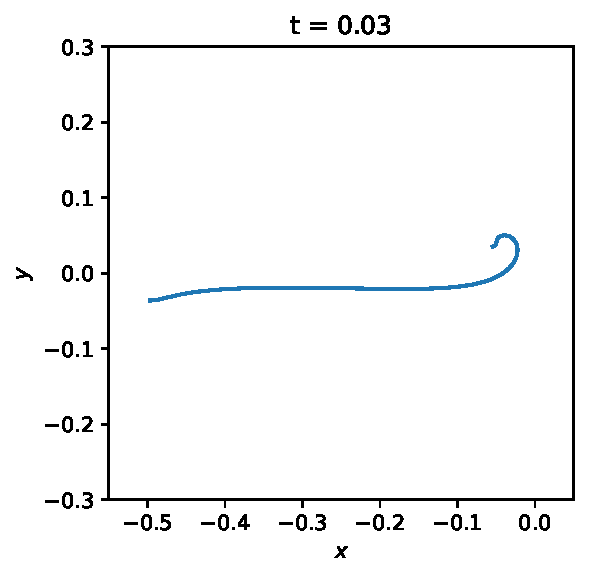
\includegraphics[width=7cm]{0.03.pdf}
	}\,
\end{figure}

\begin{figure}[htp]
	\centering
	\subfloat{
	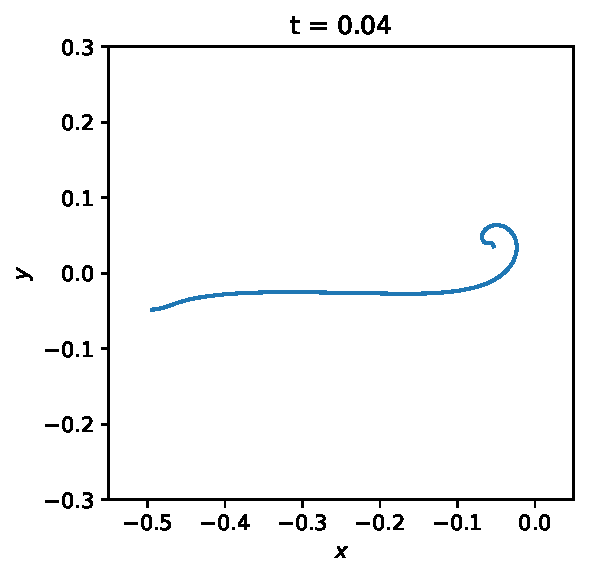
\includegraphics[width=7cm]{0.04.pdf}
	}\,
	\subfloat{
	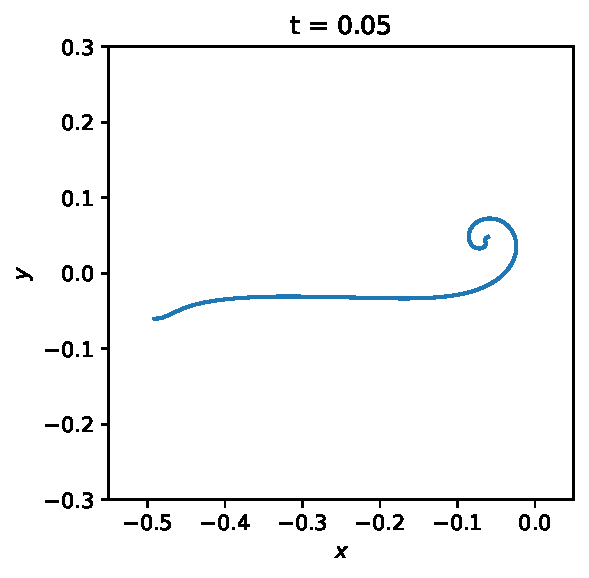
\includegraphics[width=7cm]{0.05.pdf}
	}\,
\end{figure}

\begin{figure}[htp]
	\centering
	\subfloat{
	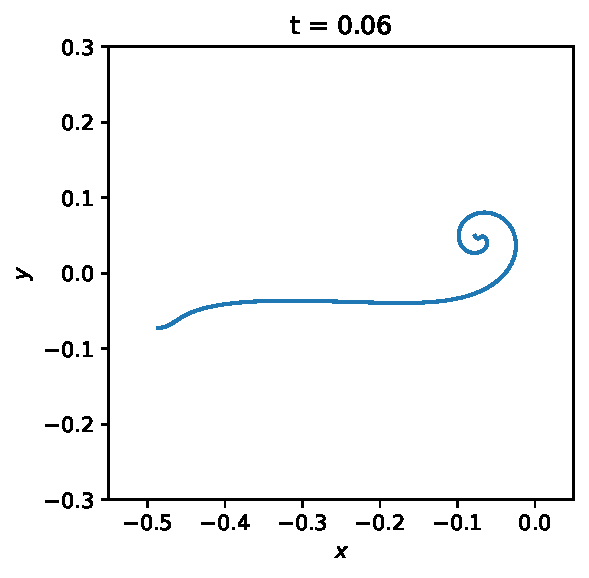
\includegraphics[width=7cm]{0.06.pdf}
	}\,
	\subfloat{
	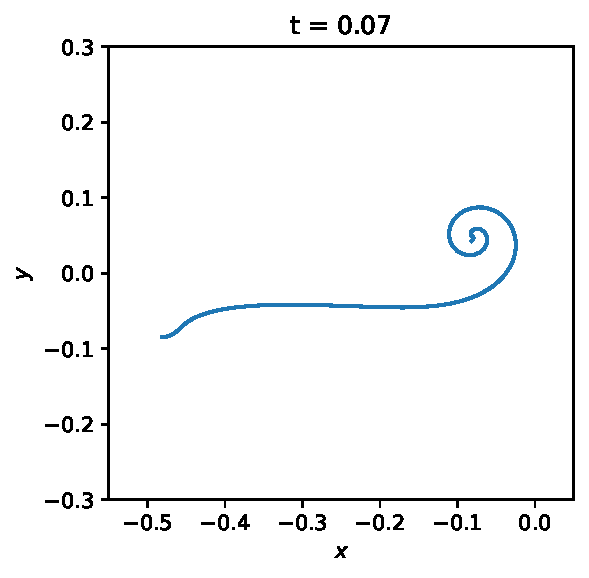
\includegraphics[width=7cm]{0.07.pdf}
	}\,
\end{figure}

\begin{figure}[htp]
	\centering
	\subfloat{
	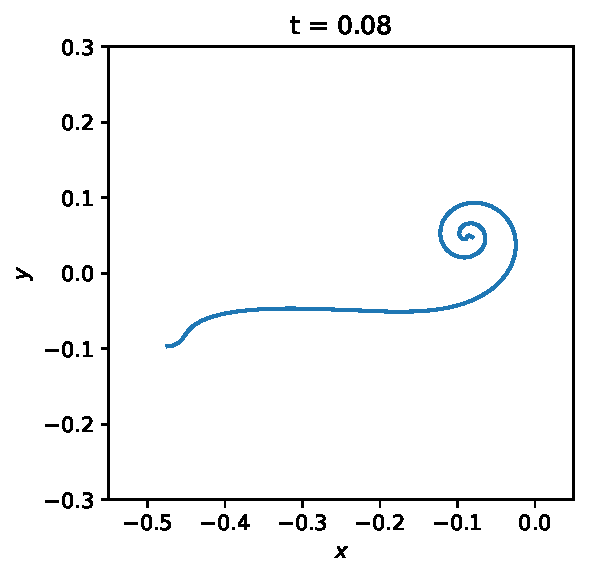
\includegraphics[width=7cm]{0.08.pdf}
	}\,
	\subfloat{
	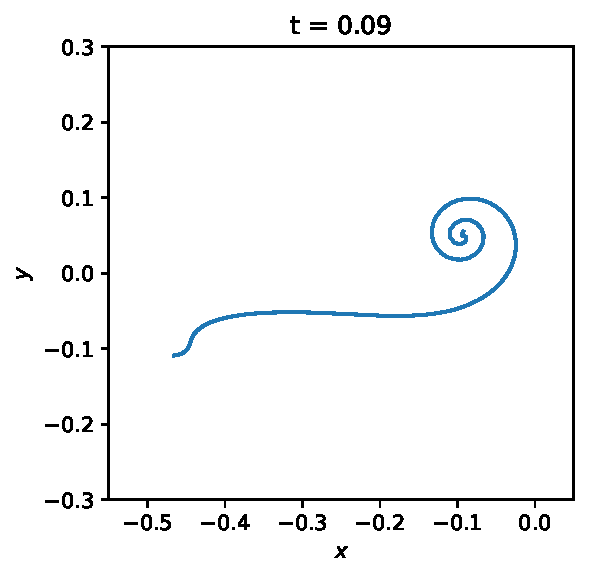
\includegraphics[width=7cm]{0.09.pdf}
	}\,
\end{figure}

\begin{lstlisting}[language={Python}]
import numpy as np
from math import cos, sin, sinh, cosh, pi, log
import matplotlib.pyplot as plt

N = 200
delta = 0.1
xmax = 0.5
n = float(N)
s = (np.arange(N) / n - 1) * xmax
dt = 0.005
T = 0.05

x = s
y = 0.0 * abs(np.flipud(s))

gamma = 1 / np.sqrt(-s)
plt.plot(gamma)
time = 0

def f1(x, y):
	dx = np.zeros(N)
	for j in range(N):
		for k in range(N):
			if k != j:
				dx[j] += sinh(2 * pi * (y[j] - y[k])) / (
					(cosh(2 * pi * (x[j] - x[k])) -
						cos(2 * pi * (y[j] - y[k])) + delta**2)) * gamma[k]
	return (-0.5 / n) * dx


def f2(x, y):
	dy = np.zeros(N)
	for j in range(N):
		for k in range(N):
			if k != j:
				dy[j] += sin(2 * pi * (x[j] - x[k])) / (
					(cosh(2 * pi * (x[j] - x[k])) -
						cos(2 * pi * (y[j] - y[k])) + delta**2)) * gamma[k]
	return (0.5 / n) * dy


xk1, yk1 = np.ones(N), np.ones(N)
xk2, yk2 = np.ones(N), np.ones(N)
xk3, yk3 = np.ones(N), np.ones(N)
xk4, yk3 = np.ones(N), np.ones(N)

Finaltime = int(T / dt)

# data = np.vstack((x, y))
for t in range(Finaltime):
	if (Finaltime - t) % 2 == 0:
		plt.figure(t)
		plt.figure(figsize=(4, 4))
		plt.xlabel(r'$x$')
		plt.ylabel(r'$y$')
		plt.title("t = %.2f" % (time))
		plt.plot(x, y)
		print(Finaltime - t)
		plt.axis([-1.1 * xmax, 0.1 * xmax, -0.6 * xmax, 0.6 * xmax])

		plt.savefig("%.2f.pdf" % (time), bbox_inches='tight')
	xk1, yk1 = x, y
	xk2 = x + 0.5 * dt * f1(xk1, yk1)
	yk2 = y + 0.5 * dt * f2(xk1, yk1)
	xk3 = x + 0.5 * dt * f1(xk2, yk2)
	yk3 = y + 0.5 * dt * f2(xk2, yk2)
	xk4 = x + dt * f1(xk3, yk3)
	yk4 = y + dt * f2(xk3, yk3)
	x = x + (dt / 6.0) * (f1(xk1, yk1) + 2 * f1(xk2, yk2) + 2 * f1(xk3, yk3) + f1(xk4, yk4))
	y = y + (dt / 6.0) * (f2(xk1, yk1) + 2 * f2(xk2, yk2) + 2 * f2(xk3, yk3) + f2(xk4, yk4))
	time += dt
\end{lstlisting}

\section{8}

\subsection{试用理论分析上一题面涡的卷绕}

\begin{equation}
	\gamma = C x^{-1/2}, \quad \Gamma = 2Cx^{1/2},
\end{equation}
其中$C$是一常数, 量纲为$L^{3/2}T^{-1}$, 面涡出事状态
\begin{equation}
	\xi(\Gamma,0) = \frac{\Gamma^2}{4C^2},\quad \Gamma \in (0,+\infty),
\end{equation}
由量纲分析
\begin{equation}
	\xi(\Gamma,t,C) = (Ct)^{2/3}f(\tau),
\end{equation}
其中
\begin{equation}
	\tau = \Gamma C^{-4/3}t^{-1/3},
\end{equation}
经过足够长时间后, 取以螺旋中心为原点的极坐标系, 通过量纲分析, 
\begin{equation}
	\Gamma(r) = 2C(\lambda r)^{1/2},
\end{equation}
其中$\lambda$是无量纲常数, 
\begin{equation}
	V_\theta = \frac{\Gamma}{2\pi r} = \frac{C \lambda^{1/2}}{\pi r^{1/2}},
\end{equation}
对于Lagrange坐标为$\Gamma_p$的某一流体质点, 
\begin{equation}
	r_p = \frac{\Gamma^2_p}{4\lambda C^2},
\end{equation}
又
\begin{equation}
	V_\theta  = r_p \left(\frac{\dif \theta}{\dif t}\right)_P,
\end{equation}
\begin{equation}
	r \approx \left(\frac{C^2\lambda}{\pi^2}\right)^{1/3} \left(\frac{t}{\theta-\theta_0}\right)^{2/3}.
\end{equation}







\nocite{*}

\bibliographystyle{plain}
\phantomsection

\addcontentsline{toc}{section}{参考文献} %向目录中添加条目,以章的名义
\bibliography{homework}

\end{document}
